\chapter{Monte Carlo Methods}
\label{chap:qmc}
\todo{...}
\todo{look especially at thijssen and the foulkes review for these sections}

% probably get some inspiration from Kai's and Werner's theses -- focus on FCIQMC

\gls{MC} methods are a class of numerical methods that use random sampling to numerically solve problems. It has found applications in an impressive range of fields, from physics to finance.\todo{citation} It is particularly useful for problems with high dimensionality, where deterministic methods are often impractical. In quantum chemistry and physics, since a `dimension' can refer to any degree of freedom, high-dimensional problems are commonplace, and so \gls{MC} methods are a natural choice.

While the name \emph{Monte Carlo} was coined by Stanislav Ulam, after the famous casino in Monaco,\todo{citation} the foundational concept was already developed in the 18th century by the French mathematician Georges-Louis Leclerc, Comte de Buffon. As one of the earliest example applications, in the Buffon needle problem, one can randomly toss needles onto a lined sheet of paper and determine $\pi$.\todo{citation}

Monte Carlo methods is a broad term, and as such it is not possible to give a comprehensive overview in a single chapter, and there exist many reviews and textbooks on \gls{MC} and related topics.\todo{citations: see those in thijssen} We will focus on only a few here concepts particularly relevant for this dissertation, largely following reference \citenum{foulkesQuantum} and the relevant chapters of \citenum{thijssenComputational2007}.

\section{Classical Monte Carlo Methods}

We start our discussion with classical \gls{MC} methods. While there are numerous possible applications, such as molecular dynamics,\todo{cite}, here we restrict ourselves to the topic of Monte Carlo integration. In particular, we consider the classical textbook problem of calculating the value of $\pi$, then we provide a more rigorous framework.

\subsection{A Very Bad Game of Darts}

If we imagine throwing darts at a dartboard randomly, we can approximate $\pi$. If the radius of the circle is $r$, then its area is $\pi r^2$. The area of the square circumscribing the circle is $4r^2$. Therefore, the ratio of the area of the circle to the area of the square is $\pi/4$. If we randomy sample a point in the square (``throw a dart''), the probability that the point is inside the circle is proportional its area. Since we sample inside the square, the probability of landing inside the circle is
\begin{equation}
    P(\text{inside circle}) =  \frac{\pi r^2}{4r^2} = \frac{\pi}{4}.
\end{equation}
Therefore, if we sample a large number of points, the ratio of the number of darts that land inside the unit circle to the total number of darts, we can approximate the probability distribution $P$ and thus get an estimate for $\pi$. This is illustrated in figure \ref{fig:darts}, and captures the core philosophy of \gls{MC} methods.

\begin{figure}[htbp]
    \centering
    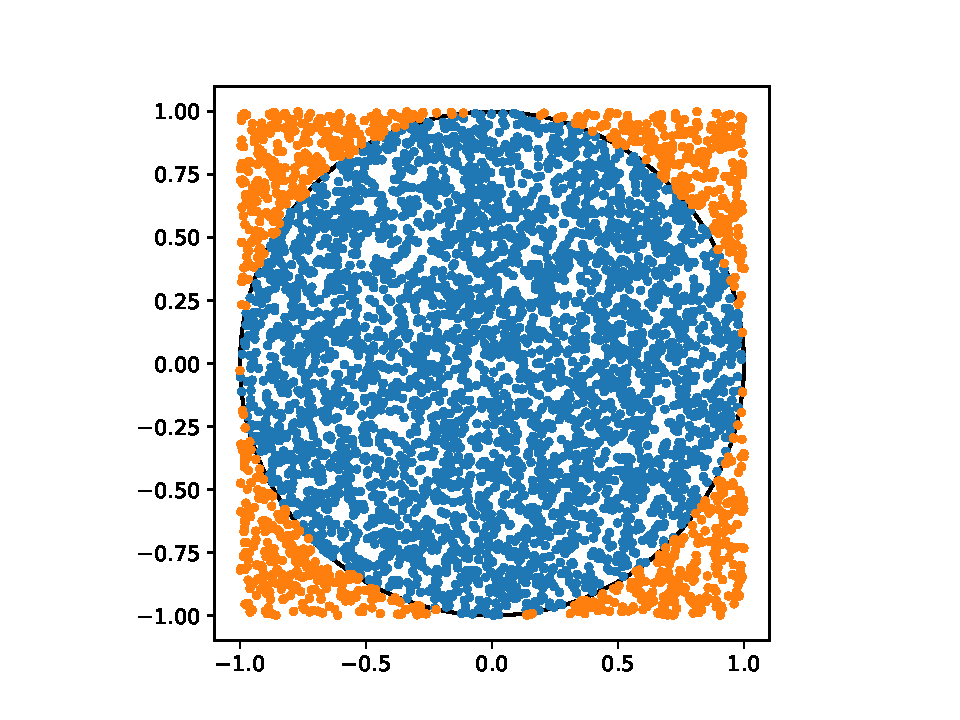
\includegraphics[width=\textwidth]{figures/qmc/darts.pdf}
    \caption{Our ``game of darts''. Points inside the unit circle are coloured blue whereas points outside are orange. Using stochastic sampling, this naive approach uses 5000 randomly generate numbers between -1 and 1 to approximate $\pi\approx 4N_\mathrm{in}/N_\mathrm{out}\approx 3.1464$. Of course, there are many ways to improve this method, the most obvious being to use a fraction of the unit circle, such as the first quadrant.}
    \label{fig:darts}
\end{figure}

\subsection{A More Mathematical Description}

As we have expressed the problem of the previous section in terms of areas, it is clear that it can also be formulated in terms of integrals. For this particular problem, we have:
\begin{equation}
    \pi = \int_{-1}^1  \mathrm{d}x \int_{-1}^1 \mathrm{d}y\ \Theta(1-x^2-y^2) ,
\end{equation}
where $\Theta$ is the Heaviside step function.
More generally, consider the integral of some smooth function $f$ over $[a,b]\subseteq \mathbb{R}$,\footnote{We present the one-dimensional case for simplicity. The generalization to higher dimensions is straightforward.}
\begin{equation}
    I = \int_a^b \d x \ f(x).
\end{equation}
Standard finite element methods for solving integrals of this type typically involving dividing the integration domain into $N$ subintervals of length $h$ and determining the weights $w_i$ from e.g. a polynomial approximation. The error $\sigma$ in these sorts of methods is typically $\sigma\propto h^{-k} \propto N^{-k}$, where $k\in\mathbb{Z}_{>0}$. For a multi-dimensional integral, $\sigma\propto N^{-k/d}$, where $d$ is the number of dimensions.\cite{ascherFirst2011}
% I am mostly following the discussion and notation in Thijssen's book -- remember to cite it along with all the primary references

In \gls{MC} methods,\todo{citations} $\forall i$ take $w_i=1$ and $x_i\in[a,b]$ randomly sampled. For uniformly sampled points, t`he variance is then
\begin{align}
    \sigma^2 &= \left\langle \left( \frac{b-a}{N}\sum^N_{i=1}f_i\right)2\right\rangle - \left( \left\langle  \frac{b-a}{N}\sum^N_{i=1}f_i\right\rangle\right)^2 \\
    &= \frac{(b-a)^2}{N}(\bar{f^2} - \bar f^2)
\end{align}
where $f_i\mathdef f(x_i)$ and $x_i$ is a random number drawn, the angular brackets denote an average over all possible realisations, and the overbar represents an average of the function over the domain ($[a,b]$ in this discussion). i.e. the error in this method is proportional to the variance of $f$. Perhaps more interestingly, $\sigma\propto N^{-1/2}$, in line with the central limit theorem.\todo{citations} Comparing this error with standard quadrature, we see that MC integration is moroe efficient than an order-$k$ algorithm when $d>2k$. That is, although this particular \gls{MC} example is naive, using simply a uniform distribution, it is still more efficient than standard methodologies for very large dimensions.

There exist several methods to reduce errors in \gls{MC} methods.\todo{citations} Among the most important ones is importance sampling. In the prevous example, it is clear that if significant contributions to the integral come from a small region of the domain, only a few points would be sampled by the \gls{MC} algorithm there. This would lead to large statistical errors. Mathematically, this is from the large variance of the function. In importance sampling, we sample from a distribution $p$ which has roughly the same shape as $f$ such that $f/p$ is roughly constant over the integration domain. Of course, being a probability distribution, we require
\begin{equation}
    p(x)>0 \quad \forall x
\end{equation}
and
\begin{equation}
    \int\d x \ p(x) = 1.
\end{equation}

The integral is
\begin{equation}
    I = \int\d x \  f(x) = \int\d x\ \frac{f(x)}{p(x)} p(x).
\end{equation}
Then, if we sample points according to $p$, we have
\begin{equation}
    I\approx \frac{1}{N}\sum^N_{i=1} \frac{f(x_i)}{p(x_i)},
\end{equation}
where the naive \gls{MC} method is recovered when $p(x)=1/(b-a)$, i.e. the uniform distribution.

In this case, the variance in the result is
\begin{equation}
    \sigma^2 = \left\langle \left( \frac{1}{N}\sum^N_{i=1} \frac{f(x_i)}{p(x_i)}\right)^2\right\rangle - \left( \left\langle  \frac{1}{N}\sum^N_{i=1} \frac{f(x_i)}{p(x_i)}\right\rangle\right)^2.
\end{equation}
From this, we can see that if $f/p$ is constant, the error vanishes, so it is important to choose a good $p$. If $p$ is chosen poorly, the variance can be worsened, so this is a delicate problem.

In practice it is often difficult to estimate $f$, and a choice for $p$ is problem-specific. However, when we have some approximation for its overall shape, importance sampling can be a powerful tool. Alternatively, another method known as adaptive Monte Carlo\todo{citation} seeks the most significant regions of $f$ by random sampling, so that no a priori knowledge of the functional form is required.

\subsection{Metropolis-Hastings Algorithm}
\label{sec:mcmc}
A particularly successful method for generating random samples $x_i$ from a probability distribution $\pi(x)$, where direct sampling of $\pi$ is difficult, is the Metropolis-Hastings algorithm.\todo{citation} Often, $\pi(x)$ is known only up to a normalisation constant, $\pi(x)=\pi(x)/C$ where $C=\int\d x\ \pi(x)$ is intractible.

The Metropolis-Hastings algorithm is based on Markov chains\todo{cite}, and we construct such a Markov chain so that its stationary distribution is $\pi(x)$, which is to say if the Markov chain starts at $\pi(x)$ for step $t$, it is still $\pi(x)$ for step $t+1$.

The probability of having a sequence of states $x_1,x_2,\ldots,x_N$ is
\begin{equation}
    p(x_1,x_2,\ldots,x_N) = p(x_1)p(x_2|x_1)p(x_3|x_2)\cdots p(x_N|x_{N-1}).
\end{equation}
where $p(x|x')$ is the transition probability from $x'\to x$. Then, the probability at step $t$ to be in state $x$, $\pi_t(x)$ is given by
\begin{equation}
\pi_{t+1}(x) = \sum_{x'\in \Omega} \pi_t(x')p(x|x')
\end{equation}
where $\Omega$ is the set of all possible states. This is called the master equation. In the stationary state, $\pi_t(x)=\pi(x)$, so
\begin{equation}
    \pi(x) = \sum_{x'\in \Omega} \pi(x')p(x|x').
\end{equation}
Finding the general solution to this problem is nontrivial. However, a sufficient (but not necessary) condition is called detailed balance:
\begin{equation}
    \pi(x)p(x|x') = \pi(x')p(x'|x).
\end{equation}
This ensures that the probability of going from $x$ to $x'$ is the same as the probability of going from $x'$ to $x$, which implies that the probability is stationary.

In order to actually construct the algorithm, we must introduce the trial step probability $\omega(x|x')$, and the acceptance probability $A(x|x')$. Then,
\begin{equation}
    p(x|x') = \omega(x|x')A(x|x').
\end{equation}
$\omega(x|x'),A(x|x')\in [0,1]$ for each pair $x,x'$, and $\sum_{x'}\omega(x|x') = 1$. Furthermore, the original formulation of the algorithm required $\omega(x|x') = \omega(x'|x)$, which leads to (plugging into the master equation)
\begin{equation}
    \frac{A(x|x')}{A(x'|x)} = \frac{\pi(x')}{\pi(x)}.
\end{equation}

The algorithm proceeds in two stages: we propose a step $x'\to x$, and then accept or reject it. The probability of accepting is
\begin{equation}
    A(x|x') = \min\left(1,\frac{\pi(x')}{\pi(x)}\right).
\end{equation}
If we accept, we set the new state to $x$, otherwise we stay at $x'$.

In practice, on a computer, accepting is done by generating a random number $r\in [0,1)$ and accepting if $r<\frac{\pi(x')}{\pi(x)}$, and otherwise rejecting. Furthermore, we don't just have a single Markov chain, but a collection of so-called ``walkers'', that each perform their own Markov chain. The integrand is then sampled at each position where the walkers reach.

One final note, is that since the current state of a Markov chain is dependent on the previous state, the Markov chain is not independent of itself. This is referred to as autocorrelation.\todo{cite} One method to reduce this autocorrelation and give essentially independent samples is known as blocking.\todo{cite}

\section{Variational (Quantum) Monte Carlo}
\label{sec:vmc}

As our first foray into \gls{QMC}, we consider \gls{VMC}. In section \ref{sec:variational_principle} we introduced the variational principle by parametrising the wave function and then finding the minimum of the expectation value of the energy occurring in the parametrisation space. If we have a large number of electrons and/or a large number of parameters, then the integrals involved in the evaluation of the energy will necessarily be high-dimensional. This is where \gls{MC} comes in. For basic trial wave functions and small atoms like Hydrogen or Helium, direct integration may be possible, but as discussed in the previous section, this quickly becomes impossible for larger systems.

For a trial wave function $\Psi$ (we omit the tilde from section \ref{sec:variational_principle}), the expectation value of the energy is
\begin{align}
    \label{eq:vmc_energy}
    \langle E \rangle &= \frac{\bra{\Psi}H\ket{\Psi}}{\bra{\Psi}\ket{\Psi}} \\
    &= \frac{\int\d^{3N}r\ \Psi^*H\Psi}{\int\d^{3N}r\ |\Psi|^2}.
\end{align}
We may calculate this integral using \gls{MC}, varying the parameters and stopping according to some minimisation algorithm. In particular, define the local energy as
\begin{equation}
    E_L(\bm r) = \frac{H\Psi}{\Psi}.
\end{equation}
Notice that the more strongly $\Psi$ resembles the exact wave function, the less strongly $E_L$ varies with $\bm r$. In particular, if $\Psi$ is equal to an exact eigenstate, then $E_L$ is constant. Therefore, an alternative objective function to the energy expectation of equation \ref{eq:vmc_energy} is the variance.\todo{cite}

Defining
\begin{equation}
    p(\bm r) = \frac{|\Psi|^2}{\int\d^{3N}r\ |\Psi|^2},
\end{equation}
we may write equation \ref{eq:vmc_energy} as
\begin{equation}
    \langle E\rangle = \frac{\int\d^{3N}r\ p(\bm r)E_L(\bm r)}{\int\d^{3N}r\ p(\bm r)}.
\end{equation}
However, $\int\d^{3N}r\ p(\bm r) = 1$ so
\begin{equation}
    \langle E\rangle = \int\d^{3N}r\ p(\bm r)E_L(\bm r).
\end{equation}

This form of the energy is amenable to the Metropolis-Hastings approach outlined in section \ref{sec:mcmc}. In principle, the algorithm is doable with just a single walker, but in practice we reduce the statistical error by using many. The algorithm then becomes

\begin{minipage}{\textwidth}
\begin{lstlisting}[escapeinside={(*}{*)}]
    Initialise (*$N$*) walkers in random positions.
    until convergence criterion met
      for each walker at position (*$r$*)
        sample the local energy (*$E_L$*) at (*$r$*)
        propose a new position (*$r'$*) with probably (*$p=|\Psi(r')/\Psi(r)|^2$ *)
        if (*$r'$*) is accepted
          set (*$r$*) to (*$r'$*)
\end{lstlisting}
\end{minipage}

The energy is then calculated as the expectation value of the local energy, averaged over the samples generated in this procedure. Steps at the beginning (before equilibrium) are discarded, and a blocking procedure should be employed. Decision to stop is generally based on compute time and/or precision required.


\subsection{Trial Functions}

While \gls{VMC} is a powerful tool, the quality of the solution is constrained by the quality of the trial wave function.

\todo{make sure to mention the Jastrow factor}
\todo{Also a section of this in Thijssen}

\section{Diffusion Monte Carlo}
\todo{main point here is just its similarity to FCIQMC}

\section{Auxiliary Field Quantum Monte Carlo}

\section{The Fermion Sign Problem}
\todo{make sure to mention the fixed node approximation here}

\section{Full Configuration Interaction Quantum Monte Carlo}
\label{sec:fciqmc}

\subsection{Main Concepts}

\subsection{Energy Estimators}

\subsection{The Sign Problem in FCIQMC}

\subsection{The Initiator Approximation}

\subsection{Reduced Density Matrix Sampling}

\subsection{Combining TC with Modern Electronic Structure}
